\section{Technical Overview}

In this section, we walk the reader through a high-level overview of corrective synchronization. We first describe the conceptual details at a technical level, and then the two main algorithmic steps and how our prototype implementation carries out these steps.

\subsection{The Concept of Corrective Synchronization}

By corrective synchronization we mean the ability to transform a concurrent run that, in its present state, may not be serializable into a serializable run. Stated formally, corrective synchronization is a relationship $h \leadsto h'$ between histories, such that (i) $h$ and $h'$ share the same initial state, and (ii) $h$ and $h'$ share the same commit log (i.e., they agree on the operations on the shared-state).

The first condition ensures that corrective synchronization yields a feasible outcome. The second is effectively the requirement not to roll back updates to the shared state. These two conditions distinguish corrective synchronization from existing solutions: Unlike pessimistic approaches, bad behaviors may occur under corrective synchronization. That is, they are not avoided, but handled as they manifest. Unlike optimistic solutions, the core handling mechanism is not to retry the transaction (or parts thereof), which implies rolling back (either committed or uncommitted) updates to the shared log, but rather to ``jump'' to another state.

\noindent \textbf{Running example.}
We illustrate the difference between corrective synchronization and classic optimistic and pessimistic synchronization in Figure \ref{Fi:motivatingOverview}, where we visually represent concurrent execution of two instances of the code listed in Figure \ref{Fi:introMotivating} using locks, STM and corrective synchronization (proceeding horizontally left-to-right). Locking serializes execution, and so there is no performance gain whatsoever. As for STM and corrective synchronization, we consider the interleaving scenario from Figure \ref{Fi:motivatingInterleaving}. 

\begin{figure*}
	\begin{center}
	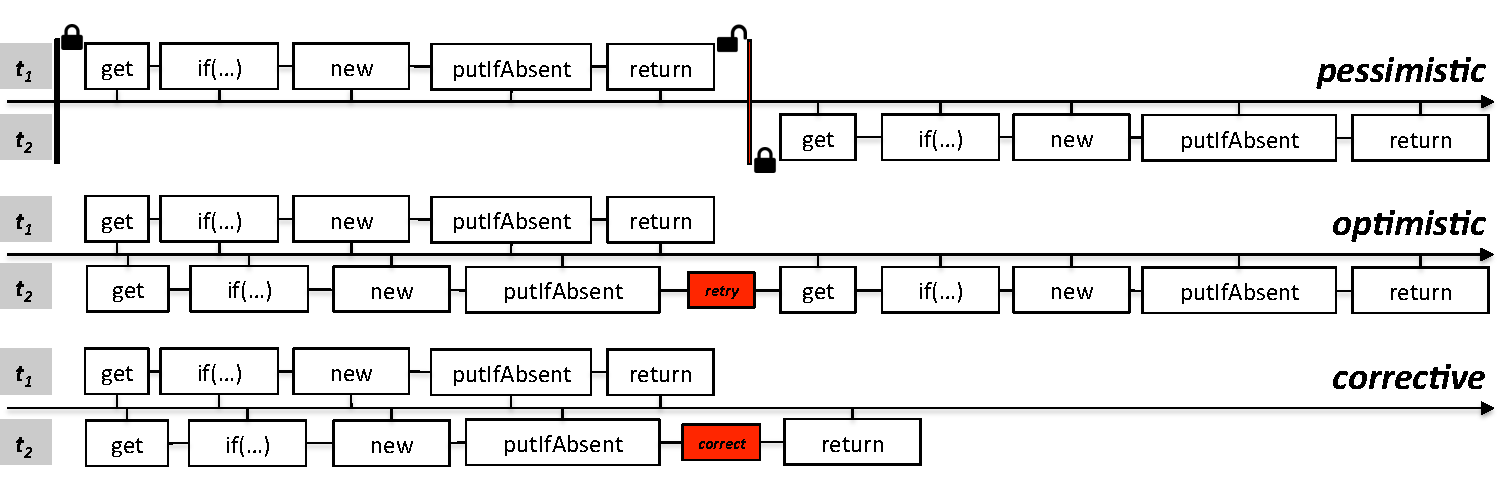
\includegraphics[width=\textwidth]{OverviewSlide.pdf}
	\end{center}
	\caption{\label{Fi:motivatingOverview}Interleaved execution of two instances of the method in Figure \ref{Fi:introMotivating} using lock-, STM- and corrective synchronization}
\end{figure*}

Both STM and corrective synchronization, allowing the problematic chain of interleavings, reach a nonserializable state. STM resolves this by retrying the entire transaction executed by thread $t_2$. This effectively yields serial execution, similarly to the lock-based run, where $t_2$ runs after $t_1$. Corrective synchronization, instead, ``fixes'' the final state, thereby allowing $t_2$ to complete without rerunning any or all of its code.

We refer to corrective synchronization as \emph{sound} if $h'$ is the prefix of a serializable execution of the system. We refer to corrective synchronization as \emph{complete} if for any $h$, all the $h'$s that satisfy the conditions above are in relation. Obviously a sound and complete corrective synchronization solution is undecidable. In the following, we describe our method of computing a sound yet incomplete set of corrective targets via static analysis of the concurrent library.

A solution that is not complete faces the problem of stuck runs. Given a (potentially) nonserializable execution prefix, the system does not have a corresponding serializable prefix to transition to. In this paper, we do not present a solution to the completeness problem, which we leave as future work. In the meantime, there are two simple strategies to tackle this problem:
\begin{compactitem}
	\item Manual specification: The user completes the set of corrective targets computed automatically, such that there are no stuck runs. In our implementation of corrective synchronization, the corrective targets are computed offline via static analysis, which lets the user complete the specification prior to the deployment runs.
	\item Complementary techniques: In the absence of a corrective target, the system can default to another synchronization technique such as STM. This provides a general means to avoid stuck states without causing any overhead w.r.t. standard techniques.
\end{compactitem}


\subsection{Computing Corrective Targets}

A simpler --- and more abstract --- specification to work with, compared to complete execution prefixes, is in the form of triplets $(s,s',s'')$ of states, such that there exist prefixes $h$ and $h'$ as above with respective initial and current states $(s,s')$ and $(s,s'')$, respectively. This form of specification is advantageous, because the runtime instrumentation it maps to is minimal compared to tracking the entire execution history. At the same time, however, merely recording initial and current states at runtime does not point back to prefixes $h$ and $h'$.

Mapping back from pairs of states to prefixes requires an oracle. In our prototype system, the oracle is computed as a relational abstract interpretation solution over the program that is sound yet incomplete. Specifically, an underapproximation of the serializable intermediate (or final) states is computed as the fixpoint solution over an interprocedural control-flow graph of the form: 
$$
	t_1 \rightarrow t^\star_{2 \ldots n} \rightarrow t_{n+1} \rightarrow t'_1 \rightarrow t'^\star_{2 \ldots n} \rightarrow t'_{n+1} \rightarrow \ldots
$$
where $t$, $t'$, etc denote different transaction types (i.e., transactions executing different code), and $n$ is unbounded, simulating a nondeterministic loop. Through this representation, we simulate an unbounded number of instances of transactions that are executed sequentially.

We go into detail about this representation in Section \ref{Se:concabs}, but note now briefly that (i) this representation reflects the effects of serial execution of the transactions, and so the corrective targets are guaranteed to be sound; (ii) the nondeterministic loop captures an unbounded number of transactions; and (iii) the first and last transactions of a given type are purposely disambiguated to boost the precision of static analysis over the simulated execution.

\noindent \textbf{Running example.} As an illustration of the third point, in our running example (Figure \ref{Fi:introMotivating}) the first transaction ( $t_1$) is modeled precisely in inserting the key/value pair into the {\sf Map} object. Analogously, the last transaction ($t_{n+1}$) can be confirmed not to update the key/value mapping.

\subsection{Runtime Synchronization} 

The runtime system has two main responsibilities. First, it must track whether execution has reached a (potentially) bad state. Second, if such a state arises, then the runtime system must map the current state onto a state that shares the same initial state and is known, by the oracle, to have a serializable continuation. 

In our implementation, the first challenge is addressed via a coarse conflict-detection algorithm that tracks API-level read/write behaviors (at the level of {\sf Map} operations). If read/write or write/write conflicts arise, then corrective synchronization is triggered in response. 

The second challenge, of deciding the target ``good'' state for a given ``bad'' state, is tackled via a lookup table that --- for a given bad state --- stores good states that can be transitioned to efficiently (that is, by applying a bounded number of state changes).

We expand on both of these challenges in Section \ref{Se:system}. Prior to that, in Sections \ref{se:instance} and \ref{sec:transactionsystemwarping}, we provide a formal statement of corrective synchronization.